\documentclass{article}
\usepackage{microtype}
\usepackage[utf8]{inputenc} 
\usepackage[a4paper, total={6in, 9.6in}]{geometry}
\usepackage{MnSymbol}
\usepackage{enumerate}
\usepackage{amsmath}
\usepackage{fancyhdr}
\usepackage{xcolor}
\usepackage{tikz}
\usepackage{pgfplots}
\usepackage{marvosym}

\widowpenalties=4 10000 10000 150 0

%% headers
\pagestyle{fancy}
\fancyhf{}
\rhead{Kommunikationssysteme WS19/20}
\lhead{Daniel Schubert, Anton Lydike}
\rfoot{Seite \thepage}

% simple command to display Aufgabe <num>)       ___ / <num>p.
\newcommand\task[1]{\section*{Aufgabe #1)\hfill \underline{\,\,\,\,\,\,}\,\,/1p.}}

% Interpretation (I)
\newcommand\I{I}
% Interpretation und belegung (I, \beta)
\newcommand\Ib{\I, \beta}

%% models
\newcommand\lmodels{\leftmodels} 			% =|
\newcommand\bimodels{\leftmodels\models}	% =||=


%% table for total points
\newcommand\pointsttl[1]{\section*{Gesamtpunkte: \hfill \underline{\,\,\,\,\,\,}\,\,/#1p.}}

%% Funktionen und Prädikate
% Funktionen (arg ist anzahl der stellen)
\newcommand\func[1]{\mathcal{F}^{#1}}
% Prädikate (arg ist anzahl der stellen)
\newcommand\praed[1]{\mathcal{P}^{#1}}

%% Regeln
\newcommand\defrule[2]{\frac{#1}{#2}}

%% Funktionszahl
\newcommand\funcnum[1]{\#_{F}\, #1}

% Für ersetzungen in belegungen wie { x \mapsto d }
\newcommand\repl[2]{\{#1 \mapsto #2\}}

% für alle x .
\newcommand\fall[1]{\forall #1 \, . \,}
\newcommand\ex[1]{\exists #1 \, . \,}

% short biimplication
\newcommand\biimpl{\Leftrightarrow}

% draw a box on the right side of the page
\newcommand\qed{ \hfill $\Box$ }

% red, green, blue text:

\definecolor{greeen}{RGB}{34,139,34}

\newcommand\red[1]{\textcolor{red}{#1}}
\newcommand\green[1]{\textcolor{greeen}{#1}}
\newcommand\blue[1]{\textcolor{blue}{#1}}

% more symbols: https://oeis.org/wiki/List_of_LaTeX_mathematical_symbols

\newcommand\cfgtitle[1]{\title{\vspace{-1.5cm}Übungsblatt #1\\%
\begin{large} Übungsgruppe Metcalfe \end{large}} \lfoot{Übungsblatt #1}\cfoot{Übungsgruppe Metcalfe}}
\author{Daniel Schubert\\Anton Lydike}


%%%%%%%%%%%%%%%%%%%%%%%
%% plotting helpers  %%
%%%%%%%%%%%%%%%%%%%%%%%

%% these draw vertical features
\newcommand\htl[1]{(#1,1) (#1,-1)}  		%% draw line from low to high
\newcommand\lth[1]{(#1,-1) (#1,1)}			%% draw line from high to low

\newcommand\sigtick[2]{\htl{#1} \lth{#2}}	%% draw a htl and then lth line

%% these draw horizontal features
\newcommand\sig[3]{(#2,#1) (#3,#1)}		%% draw a line at height #1 from x=#2 to x=#3
\newcommand\sighi[2]{\sig{1}{#1}{#2}}		%% draw a high signal from #1 to #2
\newcommand\sigmed[2]{\sig{0}{#1}{#2}}		%% draw a null signal from #1 to #2
\newcommand\siglo[2]{\sig{-1}{#1}{#2}}		%% draw a low  signal from #1 to #2


\newcommand\fakeaxis[2]{\addplot [-stealth,black] coordinates {(#1,0) (#2,0)};}



%% units
\newcommand\m{\text{ m}}
\newcommand\s{\text{ s}}
\newcommand\mps{\frac{\text{m}}{\text{s}}}
\newcommand\Gbps{\text{ Gbps}}
\newcommand\bps{\text{ bps}}
\newcommand\bit{\text{ b}}
\newcommand\B{\text{ B}}


\pgfplotsset{compat=1.15}

\renewcommand{\arraystretch}{1.5}

\newcommand\tunderset[2]{\underset{\text{#1}}{\text{#2}}}

\cfgtitle{9}
\date{Mittwoch 8.1.2020}

\begin{document}
\maketitle
\thispagestyle{fancy}

\task{1}
\begin{enumerate}[a)]
	\item Eine möglich Aufteilung des Subnetzes 100.90.80.0/20 sieht aus wie folgt: \\
	\begin{tabular}{c|c|c|c}
				Name des Subnetzes & Anzahl der IP-Adressem & Präfixnotation   & Broadcast     \\ \hline
				A 				   & 128                    & 100.90.80.0/25   & 100.90.80.127 \\
				B 				   & 1024                   & 100.90.84.0/22   & 100.90.87.255 \\
				C 				   & 2048                   & 100.90.88.0/21   & 100.90.95.255 \\
				D 				   & 512                    & 100.90.82.0/23   & 100.90.83.255 \\
				E 				   & 128                    & 100.90.80.128/25 & 100.90.80.255
		\end{tabular}
	\item Das Subnetz \texttt{2001:db8:1::/48} in acht gleichgroße Subnetze aufgeteilt. Das erste Subnetz wird notiert mit 
	\texttt{2001:db8:1::/51} und das Letzte mit \texttt{2001:db8:1:e000/51}.
	
\end{enumerate}

\task{2}
\begin{enumerate}[a)]
	
	\item \begin{itemize}
		\item \textit{ARP} wird auf L2 verwendet um Mac-Adressen zu ermitteln
		\item \textit{DHCP} wird auf L3 verwendet um neuen Hosts in einem Netzwerk 
		dynamisch eine IP-Adresse zuzuweisen.
	\end{itemize}
	
	\item 
	\begin{itemize} 
		\item Host E → Host A 
		\begin{itemize}
			\item Host E sendet IP Datengram ermittelt Mac-Adresse von Router R3
			\item Router R3 Ermittelt Mac-Adresse von Router R2
			\item Router R2 ermittelt Mac-Adresse von Host A
		\end{itemize}
		\item Host C → Host D
		\begin{itemize}
			\item Host C ermittelt Mac-Adresse von Router R2
			\item Router 2 Ermittelt Mac-Adresse von Host D
		\end{itemize}
	\end{itemize}

	\item Nach dem SLAAC verfahren, stellt gehört IPv6 Adresse \texttt{fe80::202:2ff:fe02:123} zur Mac-Adresse \texttt{00:02:02:02:01:23}
	
	\item \begin{itemize}
		\item Sende \textit{DHCP-Discover} per IP-Broadcast (Adresse 255.255.255.255)
		\item Empfange \textit{DHCP-Offer} von DHCP-Server mit konfigurationsparametern
		\item Sende \textit{DHCP-Request} um IP-Adresse zu beantragen
		\item Warte auf \textit{DHC-ACK} als aknowledgement, dass IP-Vergabe erfolgreich war
	\end{itemize}

\end{enumerate}

\pagebreak

\task{3}
\begin{enumerate}[a)]
	
	\item $$\tunderset{Label}{www}.\underset{\tunderset{Hostname}{SLD}}{example}.\tunderset{TLD}{org}$$
	
	\item \begin{itemize}
		\item \emph{Resource Records}: grundlegende Informationseinheit im DNS. \\
		   RR-Format: \texttt{<Name> <Type> <Class> <TTL> <RDLength> <RData>}
		\item Email bezogene Resource records werden mit 
	\end{itemize}
	
	\item \begin{itemize}
		\item \emph{Iterativer DNS-Lookup}: Der eingetragene DNS-Server fragt für jede Ebene des Domain-Names selbst den 
		zugehörigen DNS-Server
		\item \emph{Rekursiver DNS-Lookup}: Der DNS-Lookup-Request "läuft" an den entsprechenden DNS-Servern entlang,
		bis er beim zugehörigen Server landet, dann wird die Antwort auf dem gleichen Weg zurückübertragen.
	\end{itemize}
	
	\item Um als NAT agieren zu können, muss ein Router: 
	\begin{itemize}
		\item Die IP-Adressen des Absender- und Empfänger-Host kennen, und
		\item Das Absender- und Empfänger-Port der einzelnen Requests lesen können.
	\end{itemize}
	
	% server: 128.119.40.86
	% Host A: 192.168.1.10
	% Router: 192.168.1.1  (lokal)
	%         126.13.89.67 (public)
	\item \textbf{Pakete an den Messpunkten:} \\
		\begin{tabular}{c||c|c||c|c}
			Messpunkt & Absender IP   & Absender Port & Empfänger IP  & Empfänger Port \\ \hline
			1 (req)   & 192.168.1.10  & 1234          & 128.119.40.86 & 80             \\ 
			2 (req)   & 126.13.89.67  & 4567          & 128.119.40.86 & 80             \\ 
			3 (resp)  & 128.119.40.86 & 80            & 126.13.89.67  & 4567           \\ 
			1 (resp)  & 128.119.40.86 & 80            & 192.168.1.10  & 1234
		\end{tabular}

		\bigskip \textbf{NAT-Tabelle:} \\
		\begin{tabular}{c|c|c}
			Private IP            & Privater Port & Öffentlicher Port \\ \hline
			192.168.1.10 (Host A) & 1234          & 4567
		\end{tabular}

	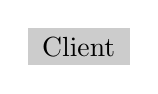
\begin{tikzpicture}
		\begin{scope}

			\draw node[rectangle,fill=black!20] (router) {Router};
			\draw node[rectangle,fill=black!20] (client) {Client};

		\end{scope}
	\end{tikzpicture}

\end{enumerate}

\pointsttl{3}


\end{document}
